\documentclass[10pt,a4paper]{book}
\usepackage[utf8]{inputenc}
\usepackage[english]{babel}
\usepackage{amsmath}
\usepackage{amsfonts}
\usepackage{amssymb}
\usepackage{graphicx}
\usepackage{physics}
\usepackage{stmaryrd}
\usepackage{tikz}

\usepackage[left=2cm,right=2cm,top=2cm,bottom=2cm]{geometry}
\author{Marco Biroli}
\title{Topology in physics}

\begin{document}
\maketitle

\chapter{Introduction}
\section{Brief introduction to topology}
\subsection{Geometry vs Topology.}

\begin{figure}[h]
\label{ex:1}
\centering
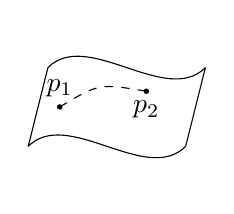
\begin{tikzpicture}
\draw (0, 0) .. controls (0.5, 0.5) and (1.5, -0.5)  .. (2, 0); 
\draw (0.25, 1) .. controls (0.75, 1.5) and (1.75, 0.5)  .. (2.25, 1);
\draw (0, 0) -- (0.25, 1);
\draw (2, 0) -- (2.25, 1);
\fill[fill=black] (0.4,0.5) node[above] {$p_1$} circle (1pt);
\fill[fill=black] (1.5,0.7) node[below] {$p_2$} circle (1pt);
\draw[dashed] (0.4, 0.5) .. controls (0.9, 0.8) .. (1.5, 0.7);
\end{tikzpicture}
\caption{A simple example of a manifold and the complexity of the notion of distance on such an object. }
\end{figure}
Take Figure \ref{ex:1} for example. A geometrical study would try to indentify local details of the structure, the radius of curvature at each point on the boundary for example. In contrast topology is only interested in the global view of the object, for example does the object contain a hole? 

\subsubsection{Local details: differential geometry}
Again we take the Figure \ref{ex:1} as reference. A common question would be for example what is the distance in between $p_1$ and $p_2$. However there is no obvious answer to such a question. One first has to define what is called a metric on the space, which is an object that will define distance in this space. The mathematical construction is written as $\dd s^2 = g_{\mu \nu} \dd x^\mu \dd x^\nu$. Let's say now that we want to compute gradients of vectors. To do such a thing one must understand how vectors change in the space. Hence we need a notion of transport for vectors. One way to do so is what is called parallel transport. The idea is to drag a vector along a path in the space to another position whilst not changing the vector. Notice in Figure \ref{parallel transport} however that parallel transport depends on the path used to transport the vector.
\begin{figure}[h] \label{parallel transport}
\centering
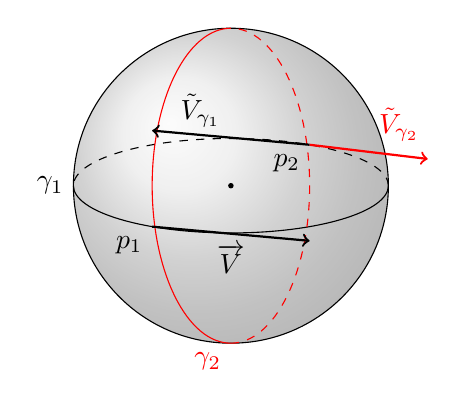
\begin{tikzpicture}
\shade[ball color = gray!40, opacity = 0.4] (0,0) circle (2cm);
  \draw (0,0) circle (2cm);
  \draw (-2,0) arc (180:360:2 and 0.6);
  \draw[dashed] (2,0) arc (0:180:2 and 0.6);
  \draw[red] (0, -2) arc (-90:90:-1 and 2);
  \draw[dashed, red] (0, -2) arc (-90:90:1 and 2);
  \draw (-2, 0) node[left] {$\gamma_1$};
  \draw (0, -2) node[below left, red] {$\gamma_2$};
  \fill[fill=black] (0,0) circle (1pt);
  \draw (-1, -0.52) node[below left] {$p_1$};
  \draw[thick, ->] (-1, -0.52) -- node[below] {${\overrightarrow{V}}$} (1, -0.7);
  \draw (1, 0.52) node[below left] {$p_2$};
  \draw[thick, ->] (1, 0.52) -- node[above left ] {$\tilde{V}_{\gamma_1}$} (-1, 0.7);
  \draw[thick, ->, red] (1, 0.52) -- node[above right] {$\tilde{V}_{\gamma_2}$} (2.5, 0.34);
\end{tikzpicture}
\caption{A simple example of mismatch under parallel transport. Notice that the vector $\vec{V}$ transported through $\gamma_1$ (resp. $\gamma_2$) leads to $\tilde{V}_{\gamma_1}$ (resp.  $\tilde{V}_{\gamma_2}$) and however $\tilde{V}_{\gamma_1} \neq  \tilde{V}_{\gamma_2}$.}
\end{figure}
This concept is called mistmatch under parallel transport. Actually the way mathematician define curvature is by saying that a vector parallely transported around a loop will be mismatched with itself.

\subsubsection{Riemann curvature tensor}
Suppose we have a very big manifold. We are now interested at what happens very close to a certain point $p$ as shown in Figure \ref{reimann-curvature}. Now at the lowest order in the perturbation we a vector $\overrightarrow{V}$ at $p$ will be deformed from $p$ to $p_{end}$ as given by:
\[
\tilde{V}^\mu_{\gamma_2} (p_{end}) - \tilde{V}^\mu_{\gamma_1}(p_{end}) \equiv V^\alpha R_{\alpha \lambda \nu}^{\mu} \varepsilon^\lambda \delta^\nu
\]
The tensor $R$ is the Reimann curvature tensor and is a local property of the manifold.

\subsubsection{Curvature of surface}
Notice now that the Reimann tensor has an upper and a lower index hence something intersting to do is to contract these indeces. In fact we have that:
\[
R_{\alpha \lambda \nu}^\mu \to R_{\alpha \lambda \nu}^\lambda = [Ric]_{\mu \nu}
\]
Which is called the Ricci tensor and is used in General Relativity. In order to introduce a scalar quantity of curvature one must use a notion of distance given by the $g^{\mu \nu}$ tensor. Which we get as:
\[
[Ric]_{\mu \nu} \to \mathcal{R} = g^{\mu \nu} [Ric]_{\mu \nu}
\] 
Which also enters into Einstein's equations. Now in the special case of 2D surface we have that:
\[
\mathcal{R} = 2 \mathcal{K} \text{ where } K \text{ is the gaussian curvature of the surface.}
\]
Hence in 2 dimensions we have an intuitive interpretation of the contraction of the Ricci tensor. 


\begin{figure} [h]
\label{reimann-curvature}
\centering
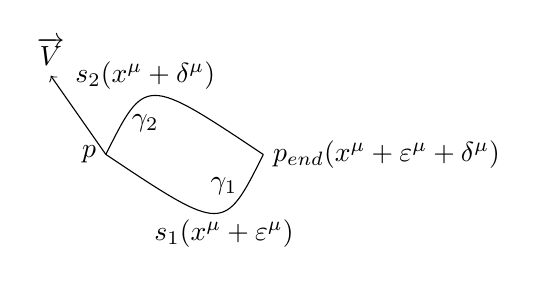
\begin{tikzpicture}
\draw (0, 0) node[left] {$p$} .. controls (0.5, 1) .. (2, 0) node[right] {$p_{end}(x^\mu + \varepsilon^\mu + \delta^\mu)$};
\draw[->] (0,0) -- (-0.7, 1) node[above] {$\overrightarrow{V}$};
\draw (0.5, 1) node {$s_2(x^\mu + \delta^\mu)$};
\draw (0.5, 0.4) node {$\gamma_2$};
\draw (0, 0) .. controls (1.5, -1)  .. (2, 0);
\draw (1.5, -1) node {$s_1(x^\mu + \varepsilon^\mu)$};
\draw (1.5, -0.4) node {$\gamma_1$};
\end{tikzpicture}
\caption{The graphical intuition behind the microscopic reasoning leading to the Riemann curvature tensor.}
\end{figure}

\subsection{Global view: topology}
The idea now with topology is to ignore local details and interest ourselves only with features that are robust against smooth perturbations. We are especially interested in classification of objects in term of their general properties. Characteristics that allow us to split objects into classes are called topological invariants and they are the quantization of the properties which are robust against smooth perturbations. An example of such an invariant for surfaces is the $\nu = $ "genus" which corresponds to the number of holes or handles. Notice that this is indeed a general property of the object and not a local one. It is however possible to connect geometrical properties to topological ones by integrating them over the manifold. This is done through the Gauss-Bonnet theorem (the following statement works only for surface without edges however it can be generalized to any manifold):
\[ 
\underbrace{\frac{1}{2\pi} \int_\mathcal{M} \mathcal{K} \dd s}_{\text{local gaussian curvature}} = \underbrace{(1 - \nu)}_{\text{global genus}}
\]

\section{Topology in electromagnetism}
\section{Berry's geometric phase}
\section{Topological Matter}
\section{Synthetic topological systems}

\end{document}